
\section{Implementation}

The classifier control loop has a target frequency of 100 $Hz$, matching the highest input frequency (joint status). 
A zero order hold is used for data streams with a lower update frequency. 
The classification is performed on matrices composed with information generated from 100 samples. 
Thus, a classification is generated every second.
In other words, every 100 samples a matrix input for the classifier is completed and a new classification is performed, which happens every 1 $s$.
Since the speed of the rover in the analyzed data sets is 0.1 $m/s$, the resolution of the categorized patches of terrain is 10 $cm$ long.  

The classification results are required frequently to allow other on-board components take advantage of the results (e.g. to improve navigation) and to ensure that the classification result corresponds to the currently traversed surface. 
Likewise, the loss of data samples due to full queues on the input of the processing components needs to be avoided. 

The diagram in Figure~\ref{fig:overview} presents the implementation approach of the terrain classifier in Rock. 
The first step, the extraction of a data sample from the relevant fields of data, is done using the \emph{type to vector} Rock tool and needs to be performed efficiently 
At each execution of the \emph{updateHook} (every 0.01 $s$) new data is stacked in the input matrix.
Every hundred \emph{updateHook} executions, an input matrix is finished and the component triggers the computation of the physical and statistical features as well as the classification itself, the \emph{prediction}.
The output of the classification and the computed features are delivered to the calling component which retrives the values through its output ports. 

\begin{figure*}[!htbp]
    \centering
    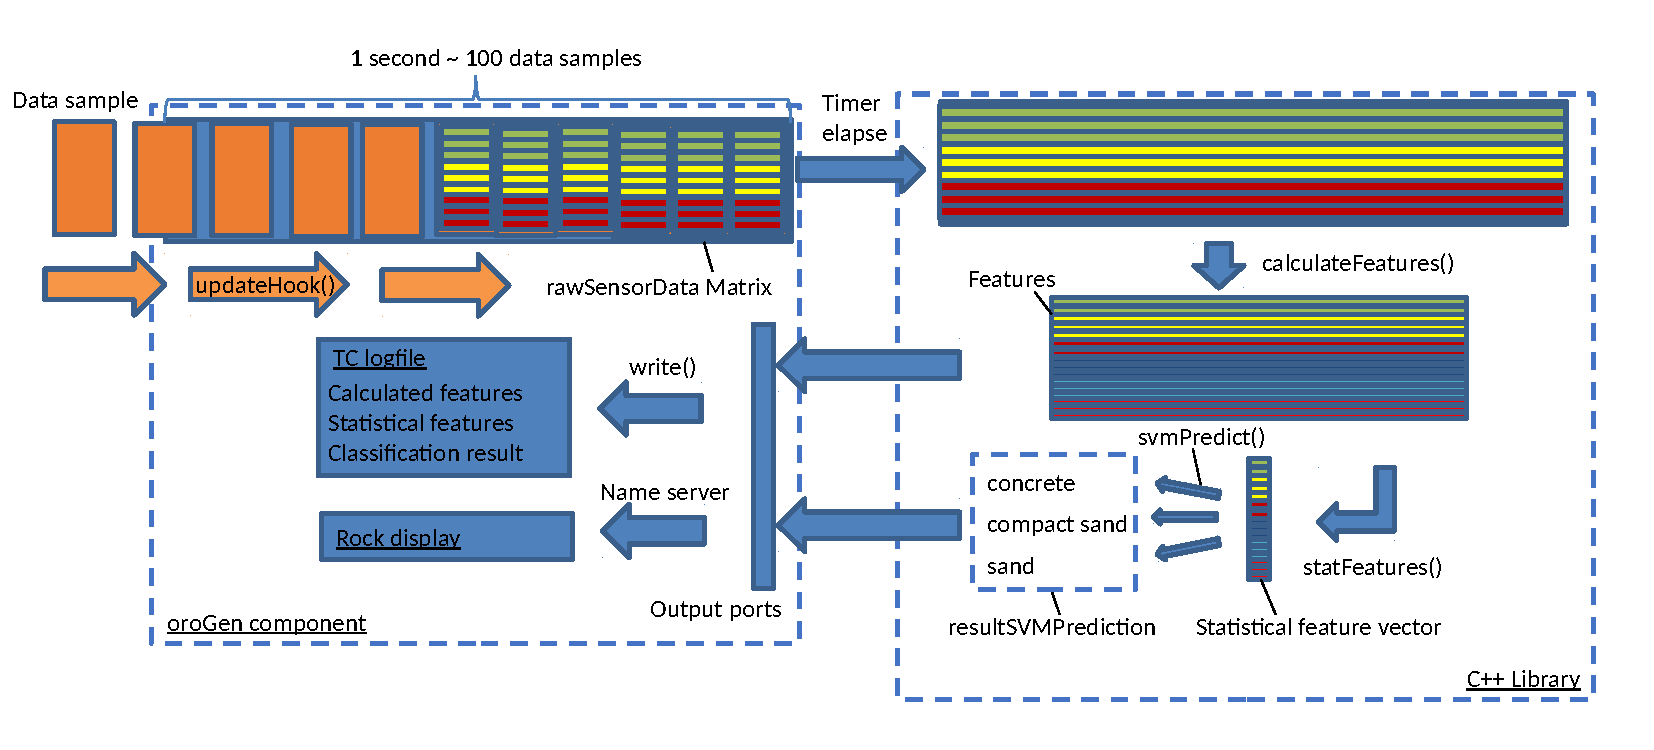
\includegraphics[width=0.9\textwidth]{../figures/OverviewTC2.pdf}
    \caption{\label{fig:overview}Overview of the terrain classifier library and Rock integration.}
\end{figure*}

\subsection{Training Data}

An essential requirement for a good classification performance is the availability of a consistent and large data collection for training and testing. 
The data collection available for this implementation consists of a dataset composed of traverses that are acquired by remotely commanding the rover over the three examined terrain types: \emph{loose sand}, \emph{compact sand} and \emph{concrete}. 
One traverse in the dataset corresponds to driving 10 $m$ forwards and backwards. 
The following conditions are kept consistent during all traverses: (1) fixed wheel configuration, (2) surfaces without inclination, (3) traverse speed of 0.1 $m/s$, (4) straight traverses and (5) the electric power generator is running, which causes vibrations.
Figure~\ref{fig:TestLocs} shows images of the rover traversing the different terrains during the data collection.


\begin{figure}[!htb]
   \centering
    \subcaptionbox
        {Loose Sand}
        {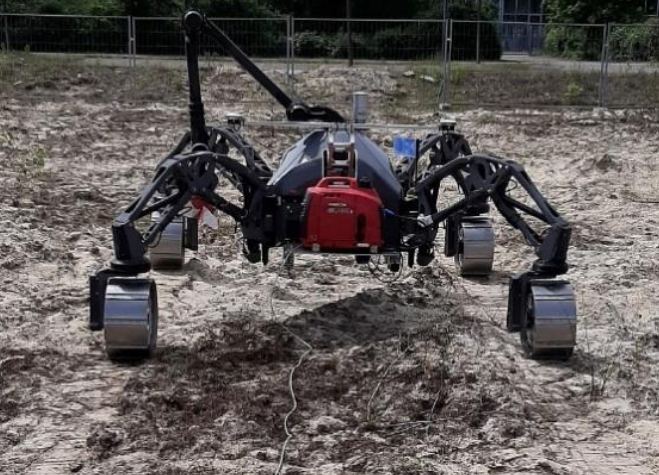
\includegraphics[width=\columnwidth]{../figures/unprepsand.png}}
    \subcaptionbox
        {Compact Sand}
        {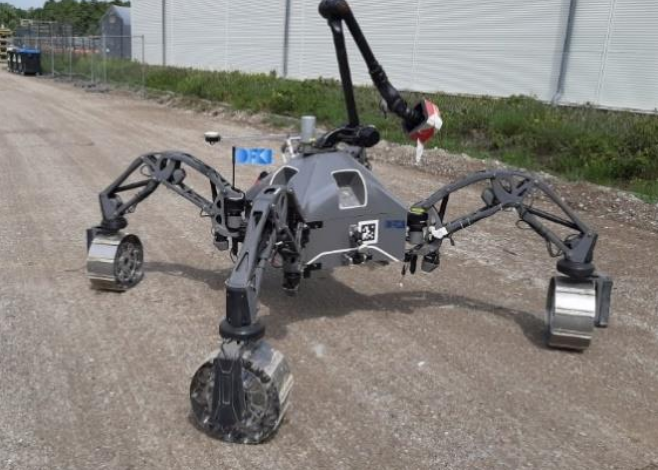
\includegraphics[width=\columnwidth]{../figures/compact.png}}
    \subcaptionbox
        {Concrete}
        {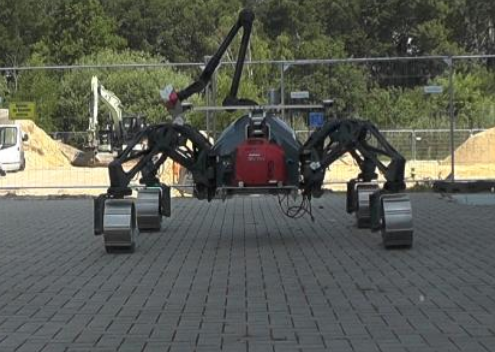
\includegraphics[width=\columnwidth]{../figures/concrete_v2.png}}
    \caption{The test locations where the data sets were acquired.}
    \label{fig:TestLocs}
\end{figure}

In terms of quantity, the data collection consists of 2200 training samples for each of the 76 features. 
Regarding data balance, the data gathered from the terrain type loose sand represents 28\%, whereas concrete and compact sand each represent 36\% of the total amount of data.
When generating a SVM model, the collected data is divided into training and testing sets. 
For the presented classifier, one of the traverses of each terrain is used for testing and all other traverses are used for training. 
This yields a ratio of about 25\%/75\%.
